\section{A Particle in an Infinite Square Well}
%By Matt Trawick

\makelabheader %(Space for student name, etc., defined in master.tex)

\bigskip

\begin{wrapfigure}[19]{r}{0.45\textwidth}
\begin{center}
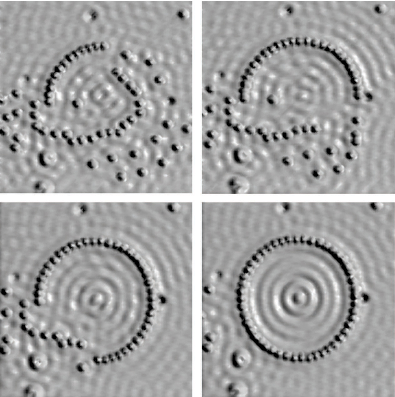
\includegraphics[width=0.42\textwidth]{particle_in_infinite_well/quantum_corral.pdf}
\end{center}
\end{wrapfigure}

\textbf{Introduction}

The image on the right shows the step by step assembly of a ring of iron atoms on a smooth copper surface.  The  electrons on the surface of the copper are confined by the iron ring in a kind of ``quantum corral'' that highlights their wavelike nature. The apparent waves you see are areas of alternating high and low density of electrons, or more accurately \textit{probability density}.  Periodic areas of high and low probability density are a common feature anytime a particle is confined to a small space, as in an electron orbiting a single atomic nucleus.  Real atoms and electrons get pretty complicated pretty fast, so today you will use both a computer simulation and direct calculation to find regions of high and low probability for a much simpler, one-dimensional version of the situation shown in this picture.

Suppose that a particle (like an electron) is confined to move in only a single dimension, along the $x$ axis.  
The probability of finding the particle between any two points $x=a$ and $x=b$ is given by 
$P_{ab} = \int_a^b P(x)  \, dx$, where $P(x)$ is the \textit{probability density} of the particle at any specific location $x$.  The probability density is related to the \textit{wave function} $\psi(x)$ for the particle by 
$P(x)=\left|\psi(x)\right|^2$, thus the probability of finding the particle between $x=a$ and $x=b$ can be expressed as
$$P_{ab} = \int_a^b \left|\psi(x)\right|^2  \, dx.$$

\textbf{Activity 1: Preliminary look at the wavefunction}
\begin{enumerate}[wide]
\item Consider a particle that is somehow constrained to move only in the $x$ direction.  It is also confined between the values of $x=0$ and $x=L$, and absolutely cannot move outside of that range.
(A macroscopic analogy for this particle in a ``one-dimensional box'' would be something like a fly stuck in a narrow glass tube that has been capped at both ends.)
\begin{enumerate}[labparts]
\item What is $\psi(x)$ for $-\infty < x < 0$?
\answerspace{0.3in}

\item What is $\psi(x)$ for $L < x < \infty$?
\answerspace{0.3in}

\item What should $\displaystyle \int_{-\infty}^\infty \left|\psi(x)\right|^2  \, dx$ be?
\answerspace{0.3in}

\item Whatever the functional form of $\psi(x)$ is inside the box, what should its value be at $x=0$ and $x=L$ in order for 
$\psi(x)$ to be continuous?
\answerspace{0.3in}
\end{enumerate}
\end{enumerate}
\pagebreak

\begin{wrapfigure}[13]{r}{0.40\textwidth}
\begin{center}
\vspace{-0.2in}
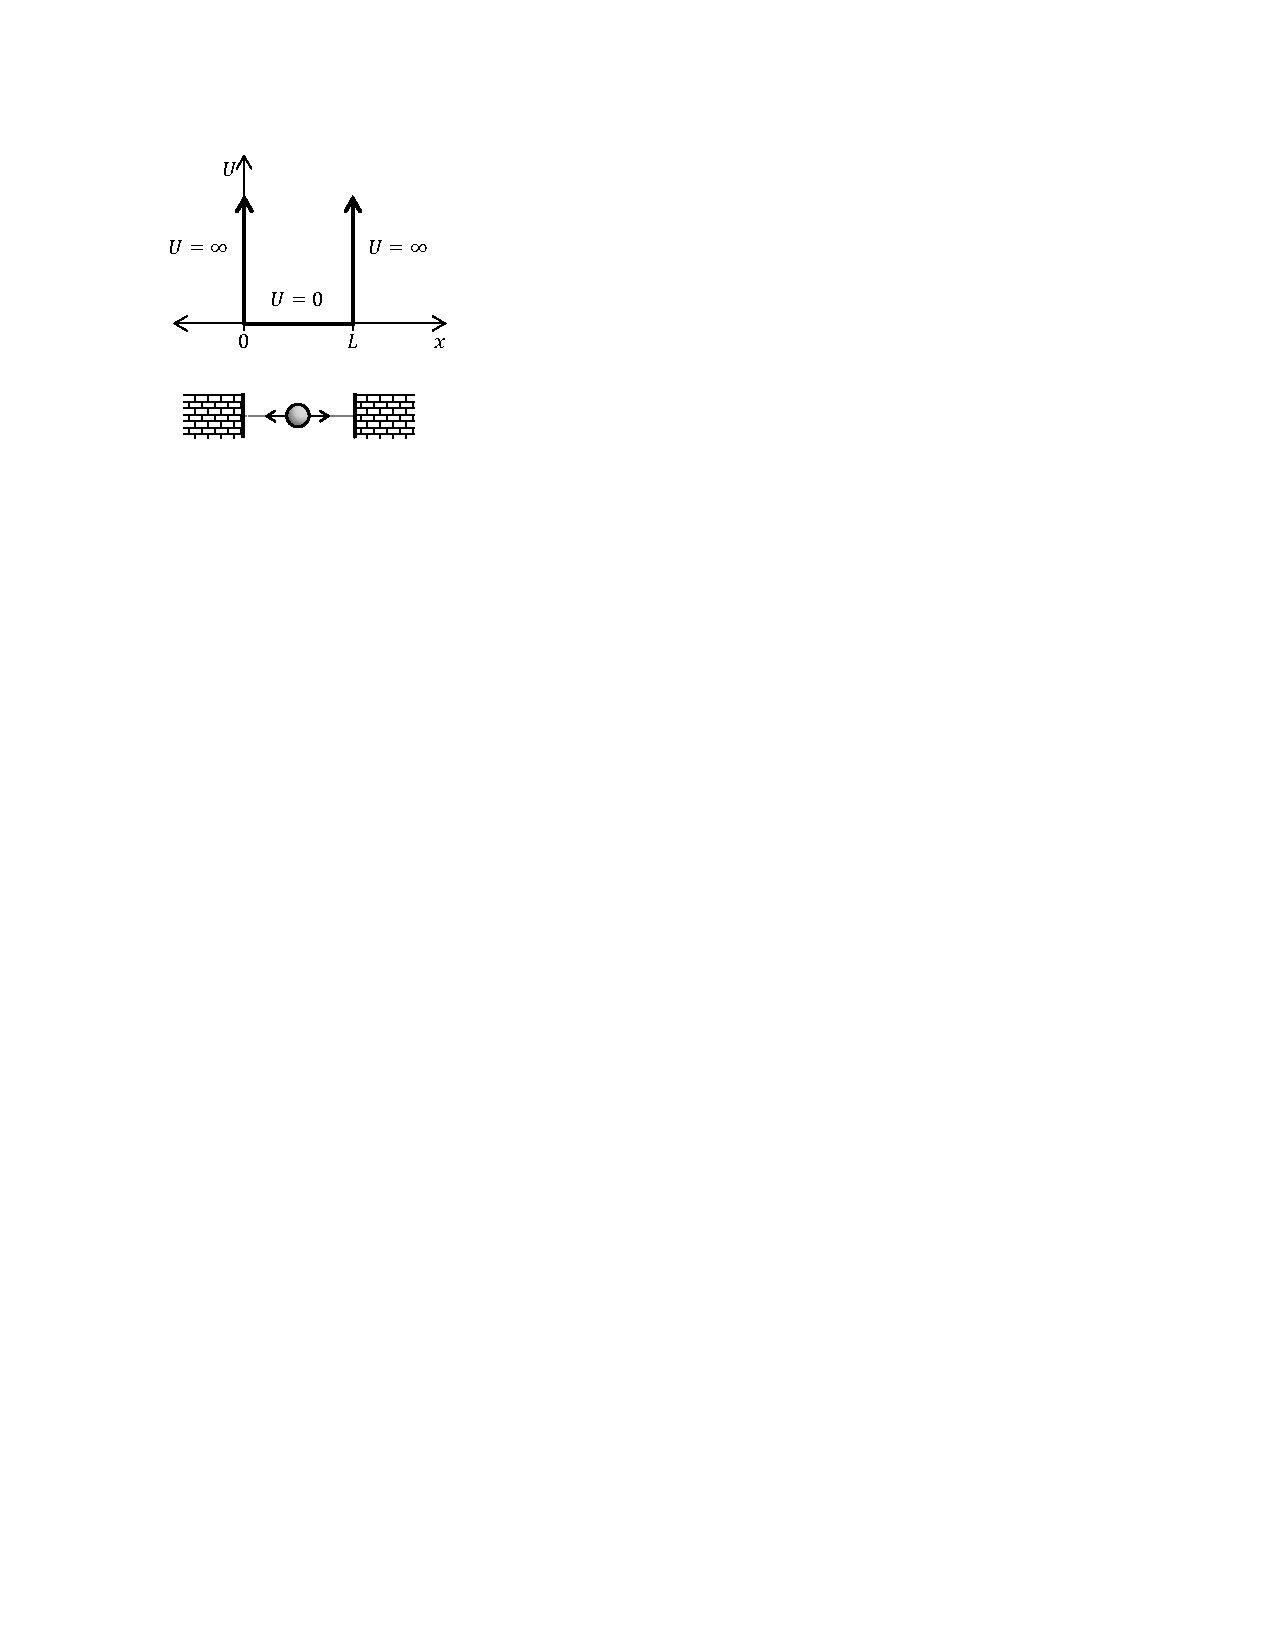
\includegraphics[width=0.34\textwidth]{particle_in_infinite_well/infinite_potential.pdf}
\end{center}
\end{wrapfigure}

%A key aspect of the Schr\"odinger equation is the interplay between the energy of the particle $E$ and the potential energy function $U(x)$, which describes the forces acting on the particle.

To calculate $\psi(x)$, we'll first have to describe the forces acting on the particle using a potential energy function $U(x)$.
For our particle trapped in a box, the potential energy, shown on the right, is an energy ``well'': high on the outsides and low in the middle.  Because the side walls of the well are vertical, we call the potential a ``square well''.  If our particle absolutely cannot move beyond the vertical walls, our particle is in an ``infinite square well'', where outside the box $U(x)=\infty$, and inside the box $U(x)=0$.

\bigskip 
Within the range $0<x<L$, you can find $\psi(x)$ using the one-dimensional, time-independent Schr\"odinger equation:
$$-\frac{\hbar^2}{2m} \frac{d^2\psi(x)}{dx^2} + U(x)\psi(x) = E\psi(x),$$
where $m$ is the mass of the particle, $E$ is its energy, and the constant $\hbar$ (pronounced ``h-bar'') is related to our old friend Planck's constant $h$ by $\hbar = {h}/{2\pi} = 1.054 \times 10^{-34}~{\rm J} \cdot {\rm s}$ (or $6.582 \times 10^{-16}~{\rm eV} \cdot {\rm s}$).
\medskip
\begin{enumerate}[wide,resume]

\item What are two kinds of functions that satisfy the Schrödinger equation inside the 1-D box? (Here, the
Schr\"odinger equation says basically that the second derivative of a function is a bunch of constants times the \textit{negative} of that same function.)
\answerspace{0.8in}

\end{enumerate}

\textbf{Activity 2: Computer Simulations}

To give yourself a preview of what $\psi(x)$ looks like for different values of energy $E$, open the
following page in Firefox:
$$\verb!https://phet.colorado.edu/en/simulation/legacy/bound-states!$$
To run the simulation, click the \textit{play} icon
($\begin{array}{l}
\includegraphics[height=3ex]{particle_in_infinite_well/play_icon.pdf}\end{array}$) 
over the image.

%Latex note: the math array above is a quick way to vertically center the inline image.

Once the simulation loads, you will need to make some adjustments to the display:
\begin{itemize}[nosep]
\item At the bottom of the screen, click the \textit{pause} button 
($\begin{array}{l}
\includegraphics[height=3ex]{particle_in_infinite_well/pause_icon.pdf}\end{array}$) 
and then click the \textit{restart} button next to it 
($\begin{array}{l}
\includegraphics[height=2.5ex]{particle_in_infinite_well/prev_track_icon.pdf}\end{array}$) 
to reset the time to $t=0$.  (In fact, we won't be messing with time evolution at all in this lab.)
\item Under ``Display'' on the right of the window, select ``Wave Function'' (not ``Probability Density'').
\item Under ``Energy chart'' at the top right, check that the ``Potential Well'' is already set to ``Square.''  
\item Click the ``Configure Potential...'' button and set the ``height'' to the maximum value of 20~eV, then click ``Close''.  In this simulation, 20~eV is as close to $\infty$ as we can get.  :-|
\item If at any time the simulation seems to misbehave or not respond, you can always hit the ``Reset All'' button and start again. 
\end{itemize}

\begin{enumerate}[wide]
\item The simulation should be showing the situation for a particle in the potential well with the \textit{lowest} energy that the particle can have, $E_1$.  You can tell because the lower graph, labeled ``Wave Function,'' shows ``$\psi_1(x,t)$'' in the legend in the upper right corner.  Also, the upper graph, labeled ``Energy (eV)'' has the lowest horizontal line highlighted in red.  When you hover your mouse over that lowest horizontal line, what is the value of the energy $E_1$ shown?
\answerspace{0.5in}

\item You said in Activity~1 that outside of the potential well, the wave function should be zero.  Is the graph of $\psi_1(x,t)$ shown consistent with that prediction?
\answerspace{0.3in}


\item Click on the horizontal lines in the upper graph to change the energy of the particle.  In the space below, draw  sketches of the wavefunctions for the lowest three possible energies, $E_1$, $E_2$, and $E_3$.  Be sure to show where $\psi = 0$ is on your vertical axis.  On your horizontal axis, make your potential well extend from $x=0$ to $x=L$ (unlike the simulation, where the well extends from $x = -0.5$~nm to $x=+0.5$~nm). 
%\answerspace{2.0in}
\vfill

\item When the energy of the particle increases, does the wavelength of the particle \textit{increase} or \textit{decrease}?
\answerspace{0.3in}

\item The wavefunction $\psi(x)$ must always be continuous over all $x$, including at the boundaries of the well.  Are all of your graphs of $\psi(x)$ above continuous everywhere?
\answerspace{0.3in}

\item Suppose you tried to graph $\psi(x)$ for an energy $E$ between $E_2$ and $E_3$ (say, $E=2.0$~eV).  Would that lead to a wave function that was continuous at both $x=0$ and $x=L$?
\answerspace{0.3in}

\item Now let's turn our attention to the probability density for the particle, $P(x)=\left|\psi(x)\right|^2$.  In the space below, use dotted lines to sketch three graphs predicting what the probability densities $P(x)$ should look like for the lowest three possible energies, $E_1$, $E_2$, and $E_3$.  As before, take care to label $P(x)=0$ on your vertical axes, and also $x=0$ and $x=L$ on your horizontal axes.
\answerspace{2.0in}


\pagebreak

\item Use the simulation to check your prediction above, by selecting ``Probability Density'' instead of ``Wave Function'' under \textit{Display}.  Use solid lines to make any corrections to your graphs above, and note below any differences.  (Note: look carefully in the simulation at places on the graphs where $P(x)$ is nearly zero.  Is the slope of $P(x)$ ever discontinuous?)
\answerspace{0.5in}
\end{enumerate}


\textbf{Activity 3: Deriving the Energies}

The computer simulation has shown that only certain, discrete values of energy $E$ lead to a wave function $\psi(x)$ that is continuous at the boundaries of an infinite square well.  In this section we will derive an algebraic expression for those allowable energies.

\begin{enumerate}[wide]
\item In Activity 1, question 2, you probably wrote that a function like either $\cos(kx)$ or $\sin(kx)$ will satisfy the Schr\"odinger equation inside the well. However, it turns out that only one of those two is guaranteed to be continuous at both $x=0$ and $x=L$.  Which one?
\answerspace{0.3in}

\item What values must $k$ have (in terms of $\pi$, $L$, and an arbitrary integer $n=1,2,3...$) such that $\psi(x)$ is guaranteed to be continuous at $x=L$?  
\answerspace{0.3in}

\item Now use the Schr\"odinger equation and take the derivatives to write an expression for the allowed values of $E$ in terms of $h$, $m$, $L$, and some integer $n$.  
\answerspace{2.0in}
\end{enumerate}

\textit{We have derived that the energy is quantized!  In classical mechanics we could give a bound particle any energy we wanted.  But because of the wave-like properties of particles in quantum mechanics, the boundary conditions placed on the wave function mean that only certain discrete values of energy are possible!}

\pagebreak

\textbf{Activity 4: Normalization Constant and Probabilities}
\begin{enumerate}[wide]

\item If you write the full wave function $\psi(x)$ for a particle in a 1-dimensional box, there is actually an arbitrary constant $A$ in front of it:
$$\psi(x)=A\sin kx$$
Use your answers to Activity 1, question 1, to find the value of $A$ (in terms of $L$) for $n=1$.  
Hint: you may find the following integral handy: $\int \sin^2ax \, dx = \frac{x}{2} -\frac{1}{4a}\sin 2ax $.

\vfill

\item What's $A$ for $n=2$?  For $n=3$?  Do you see a pattern?

\vfill

\pagebreak
\item If your particle has $n=2$, what is the exact probability of finding it between $x=0$ and $x=0.25L$?  Is your calculated answer consistent with your graphs in Activity 2?
\answerspace{2in}

\item If your particle has $n=1$, what is the exact probability of finding it between $x=0$ and $x=0.25L$?  Again, is your calculated answer plausibly consistent with your graphs in Activity 2?
\answerspace{2in}

\end{enumerate}



